% Options for packages loaded elsewhere
\PassOptionsToPackage{unicode}{hyperref}
\PassOptionsToPackage{hyphens}{url}
\PassOptionsToPackage{dvipsnames,svgnames,x11names}{xcolor}
%
\documentclass[
  letterpaper,
  DIV=11,
  numbers=noendperiod,
  oneside]{scrartcl}

\usepackage{amsmath,amssymb}
\usepackage{iftex}
\ifPDFTeX
  \usepackage[T1]{fontenc}
  \usepackage[utf8]{inputenc}
  \usepackage{textcomp} % provide euro and other symbols
\else % if luatex or xetex
  \usepackage{unicode-math}
  \defaultfontfeatures{Scale=MatchLowercase}
  \defaultfontfeatures[\rmfamily]{Ligatures=TeX,Scale=1}
\fi
\usepackage{lmodern}
\ifPDFTeX\else  
    % xetex/luatex font selection
\fi
% Use upquote if available, for straight quotes in verbatim environments
\IfFileExists{upquote.sty}{\usepackage{upquote}}{}
\IfFileExists{microtype.sty}{% use microtype if available
  \usepackage[]{microtype}
  \UseMicrotypeSet[protrusion]{basicmath} % disable protrusion for tt fonts
}{}
\makeatletter
\@ifundefined{KOMAClassName}{% if non-KOMA class
  \IfFileExists{parskip.sty}{%
    \usepackage{parskip}
  }{% else
    \setlength{\parindent}{0pt}
    \setlength{\parskip}{6pt plus 2pt minus 1pt}}
}{% if KOMA class
  \KOMAoptions{parskip=half}}
\makeatother
\usepackage{xcolor}
\usepackage[left=1in,marginparwidth=2.0666666666667in,textwidth=4.1333333333333in,marginparsep=0.3in]{geometry}
\setlength{\emergencystretch}{3em} % prevent overfull lines
\setcounter{secnumdepth}{-\maxdimen} % remove section numbering
% Make \paragraph and \subparagraph free-standing
\ifx\paragraph\undefined\else
  \let\oldparagraph\paragraph
  \renewcommand{\paragraph}[1]{\oldparagraph{#1}\mbox{}}
\fi
\ifx\subparagraph\undefined\else
  \let\oldsubparagraph\subparagraph
  \renewcommand{\subparagraph}[1]{\oldsubparagraph{#1}\mbox{}}
\fi


\providecommand{\tightlist}{%
  \setlength{\itemsep}{0pt}\setlength{\parskip}{0pt}}\usepackage{longtable,booktabs,array}
\usepackage{calc} % for calculating minipage widths
% Correct order of tables after \paragraph or \subparagraph
\usepackage{etoolbox}
\makeatletter
\patchcmd\longtable{\par}{\if@noskipsec\mbox{}\fi\par}{}{}
\makeatother
% Allow footnotes in longtable head/foot
\IfFileExists{footnotehyper.sty}{\usepackage{footnotehyper}}{\usepackage{footnote}}
\makesavenoteenv{longtable}
\usepackage{graphicx}
\makeatletter
\def\maxwidth{\ifdim\Gin@nat@width>\linewidth\linewidth\else\Gin@nat@width\fi}
\def\maxheight{\ifdim\Gin@nat@height>\textheight\textheight\else\Gin@nat@height\fi}
\makeatother
% Scale images if necessary, so that they will not overflow the page
% margins by default, and it is still possible to overwrite the defaults
% using explicit options in \includegraphics[width, height, ...]{}
\setkeys{Gin}{width=\maxwidth,height=\maxheight,keepaspectratio}
% Set default figure placement to htbp
\makeatletter
\def\fps@figure{htbp}
\makeatother
\newlength{\cslhangindent}
\setlength{\cslhangindent}{1.5em}
\newlength{\csllabelwidth}
\setlength{\csllabelwidth}{3em}
\newlength{\cslentryspacingunit} % times entry-spacing
\setlength{\cslentryspacingunit}{\parskip}
\newenvironment{CSLReferences}[2] % #1 hanging-ident, #2 entry spacing
 {% don't indent paragraphs
  \setlength{\parindent}{0pt}
  % turn on hanging indent if param 1 is 1
  \ifodd #1
  \let\oldpar\par
  \def\par{\hangindent=\cslhangindent\oldpar}
  \fi
  % set entry spacing
  \setlength{\parskip}{#2\cslentryspacingunit}
 }%
 {}
\usepackage{calc}
\newcommand{\CSLBlock}[1]{#1\hfill\break}
\newcommand{\CSLLeftMargin}[1]{\parbox[t]{\csllabelwidth}{#1}}
\newcommand{\CSLRightInline}[1]{\parbox[t]{\linewidth - \csllabelwidth}{#1}\break}
\newcommand{\CSLIndent}[1]{\hspace{\cslhangindent}#1}

\usepackage{booktabs}
\usepackage{longtable}
\usepackage{array}
\usepackage{multirow}
\usepackage{wrapfig}
\usepackage{float}
\usepackage{colortbl}
\usepackage{pdflscape}
\usepackage{tabu}
\usepackage{threeparttable}
\usepackage{threeparttablex}
\usepackage[normalem]{ulem}
\usepackage{makecell}
\usepackage{xcolor}
\KOMAoption{captions}{tableheading}
\makeatletter
\makeatother
\makeatletter
\makeatother
\makeatletter
\@ifpackageloaded{caption}{}{\usepackage{caption}}
\AtBeginDocument{%
\ifdefined\contentsname
  \renewcommand*\contentsname{Table of contents}
\else
  \newcommand\contentsname{Table of contents}
\fi
\ifdefined\listfigurename
  \renewcommand*\listfigurename{List of Figures}
\else
  \newcommand\listfigurename{List of Figures}
\fi
\ifdefined\listtablename
  \renewcommand*\listtablename{List of Tables}
\else
  \newcommand\listtablename{List of Tables}
\fi
\ifdefined\figurename
  \renewcommand*\figurename{Figure}
\else
  \newcommand\figurename{Figure}
\fi
\ifdefined\tablename
  \renewcommand*\tablename{Table}
\else
  \newcommand\tablename{Table}
\fi
}
\@ifpackageloaded{float}{}{\usepackage{float}}
\floatstyle{ruled}
\@ifundefined{c@chapter}{\newfloat{codelisting}{h}{lop}}{\newfloat{codelisting}{h}{lop}[chapter]}
\floatname{codelisting}{Listing}
\newcommand*\listoflistings{\listof{codelisting}{List of Listings}}
\makeatother
\makeatletter
\@ifpackageloaded{caption}{}{\usepackage{caption}}
\@ifpackageloaded{subcaption}{}{\usepackage{subcaption}}
\makeatother
\makeatletter
\@ifpackageloaded{tcolorbox}{}{\usepackage[skins,breakable]{tcolorbox}}
\makeatother
\makeatletter
\@ifundefined{shadecolor}{\definecolor{shadecolor}{rgb}{.97, .97, .97}}
\makeatother
\makeatletter
\makeatother
\makeatletter
\@ifpackageloaded{sidenotes}{}{\usepackage{sidenotes}}
\@ifpackageloaded{marginnote}{}{\usepackage{marginnote}}
\makeatother
\makeatletter
\makeatother
\ifLuaTeX
  \usepackage{selnolig}  % disable illegal ligatures
\fi
\IfFileExists{bookmark.sty}{\usepackage{bookmark}}{\usepackage{hyperref}}
\IfFileExists{xurl.sty}{\usepackage{xurl}}{} % add URL line breaks if available
\urlstyle{same} % disable monospaced font for URLs
\hypersetup{
  pdftitle={Report on the use of passive acoustic monitoring in Kluane National Park Reserve},
  pdfauthor={Alex MacPhail},
  colorlinks=true,
  linkcolor={blue},
  filecolor={Maroon},
  citecolor={Blue},
  urlcolor={Blue},
  pdfcreator={LaTeX via pandoc}}

\title{Report on the use of passive acoustic monitoring in Kluane
National Park Reserve}
\author{Alex MacPhail}
\date{2024-04-04}

\begin{document}
\maketitle
\ifdefined\Shaded\renewenvironment{Shaded}{\begin{tcolorbox}[frame hidden, interior hidden, breakable, enhanced, boxrule=0pt, sharp corners, borderline west={3pt}{0pt}{shadecolor}]}{\end{tcolorbox}}\fi

\renewcommand*\contentsname{Table of contents}
{
\hypersetup{linkcolor=}
\setcounter{tocdepth}{3}
\tableofcontents
}
\begin{figure}

{\centering 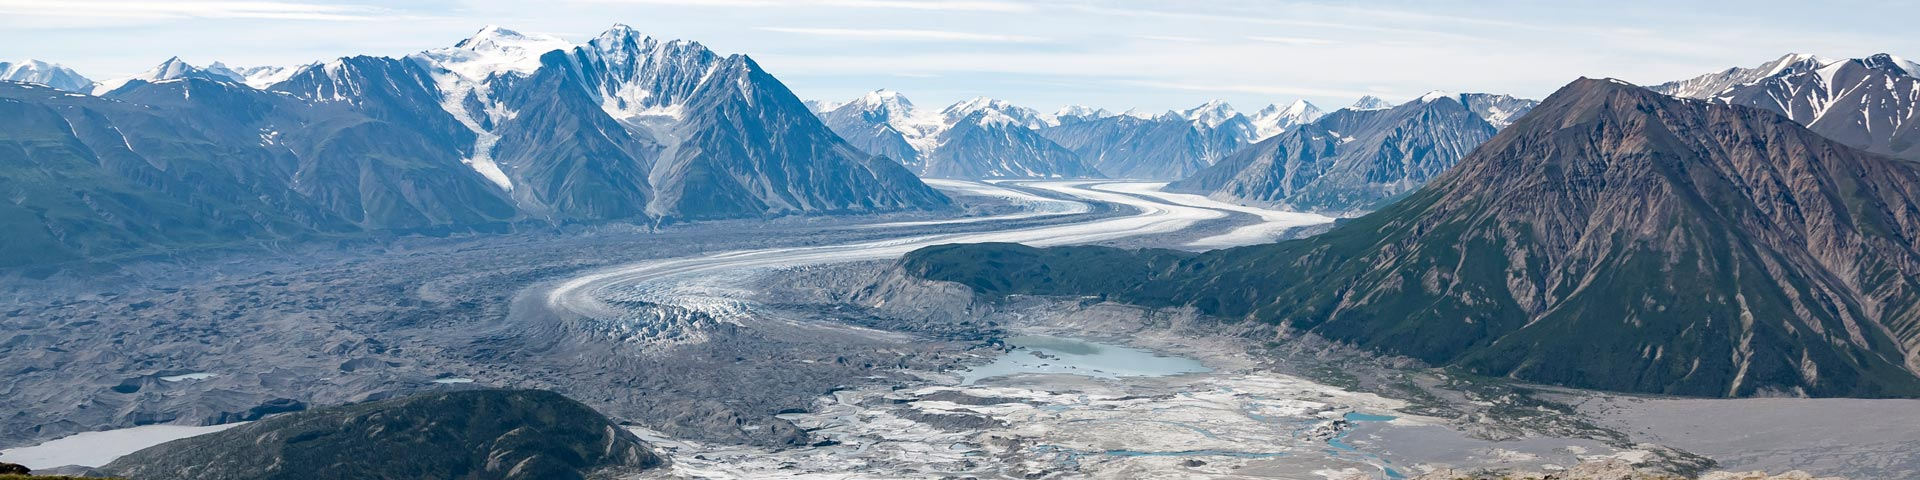
\includegraphics{kluane-banner.jpg}

}

\end{figure}

\hypertarget{abstract}{%
\section{Abstract}\label{abstract}}

Passive acoustic monitoring has proven to be a valuable tool for
monitoring vocalizing species. Environmental sensors are becoming
increasingly easy to program and can autonomously generate extensive
data sets of the soundscape, becoming an invaluable resource for
ecological integrity monitoring. Kluane National Park Reserve deployed
autonomous recording units (ARUs) across 10 locations, participated in
the national Prescribed Burn protocol. ARUs detected a total of 16
species including birds, amphibians and mammals. Despite failures from 2
locations, the analysis revealed\ldots{}

\hypertarget{land-acknowledgement}{%
\section{Land Acknowledgement}\label{land-acknowledgement}}

In the spirit of Reconciliation, we respectfully acknowledge that the
lands of Kluane National Park Reserve where this study took place are
the traditional territories of the Southern Tutchone people represented
in the Kluane region by the Champagne and Aishihik First Nations and the
Kluane First Nation. Champagne and Aishihik First Nations, Kluane First
Nation and Parks Canada are jointly responsible for the management of
Kluane's natural and cultural resources.

\hypertarget{introduction}{%
\section{Introduction}\label{introduction}}

Human activities have been identified as key pressures and contributors
to the global decline in forest wildlife (Allan et al.
(2017)\marginpar{\begin{footnotesize}\leavevmode\vadjust pre{\protect\hypertarget{ref-allan2017recent}{}}%
Allan, James R, Oscar Venter, Sean Maxwell, Bastian Bertzky, Kendall
Jones, Yichuan Shi, and James EM Watson. 2017. {``Recent Increases in
Human Pressure and Forest Loss Threaten Many Natural World Heritage
Sites.''} \emph{Biological Conservation} 206: 47--55.\vspace{2mm}\par\end{footnotesize}}).
The repercussions of habitat fragmentation (Fahrig
(2003)\marginpar{\begin{footnotesize}\leavevmode\vadjust pre{\protect\hypertarget{ref-fahrig2003effects}{}}%
Fahrig, Lenore. 2003. {``Effects of Habitat Fragmentation on
Biodiversity.''} \emph{Annual Review of Ecology, Evolution, and
Systematics} 34 (1): 487--515.\vspace{2mm}\par\end{footnotesize}})
and loss (Hanski
(2011)\marginpar{\begin{footnotesize}\leavevmode\vadjust pre{\protect\hypertarget{ref-hanski2011habitat}{}}%
Hanski, Ilkka. 2011. {``Habitat Loss, the Dynamics of Biodiversity, and
a Perspective on Conservation.''} \emph{Ambio} 40 (3): 248--55.\vspace{2mm}\par\end{footnotesize}}),
climate change (Mantyka-pringle, Martin, and Rhodes
(2012)\marginpar{\begin{footnotesize}\leavevmode\vadjust pre{\protect\hypertarget{ref-mantyka2012interactions}{}}%
Mantyka-pringle, Chrystal S, Tara G Martin, and Jonathan R Rhodes. 2012.
{``Interactions Between Climate and Habitat Loss Effects on
Biodiversity: A Systematic Review and Meta-Analysis.''} \emph{Global
Change Biology} 18 (4): 1239--52.\vspace{2mm}\par\end{footnotesize}},
Sattar et al.
(2021)\marginpar{\begin{footnotesize}\leavevmode\vadjust pre{\protect\hypertarget{ref-sattar2021review}{}}%
Sattar, Q, ME Maqbool, R Ehsan, S Akhtar, Q Sattar, ME Maqbool, R Ehsan,
and S Akhtar. 2021. {``Review on Climate Change and Its Effect on
Wildlife and Ecosystem.''} \emph{Open J Environ Biol} 6 (1): 008--14.\vspace{2mm}\par\end{footnotesize}},
Abrahms et al.
(2023)\marginpar{\begin{footnotesize}\leavevmode\vadjust pre{\protect\hypertarget{ref-abrahms2023climate}{}}%
Abrahms, Briana, Neil H Carter, TJ Clark-Wolf, Kaitlyn M Gaynor, Erik
Johansson, Alex McInturff, Anna C Nisi, Kasim Rafiq, and Leigh West.
2023. {``Climate Change as a Global Amplifier of Human--Wildlife
Conflict.''} \emph{Nature Climate Change} 13 (3): 224--34.\vspace{2mm}\par\end{footnotesize}}),
and increased access to sensitive areas exert direct and indirect
pressures on forest biodiversity, particularly in managed regions in
Canada (Lemieux et al.
(2011)\marginpar{\begin{footnotesize}\leavevmode\vadjust pre{\protect\hypertarget{ref-lemieux2011state}{}}%
Lemieux, Christopher J, Thomas J Beechey, Daniel J Scott, and Paul A
Gray. 2011. {``The State of Climate Change Adaptation in Canada's
Protected Areas Sector.''} \emph{The Canadian Geographer/Le G{é}ographe
Canadien} 55 (3): 301--17.\vspace{2mm}\par\end{footnotesize}}).
In 2023, Kluane National Park Reserve initiated a program incorporating
autonomous recording units (ARUs) for passive acoustic monitoring (PAM)
of the Park's wildlife. ARUs are compact environmental sensors that are
designed to passively record the environment (Shonfield and Bayne
(2017)\marginpar{\begin{footnotesize}\leavevmode\vadjust pre{\protect\hypertarget{ref-aru-overview}{}}%
Shonfield, Julia, and Erin M Bayne. 2017. {``Autonomous Recording Units
in Avian Ecological Research: Current Use and Future Applications.''}
\emph{Avian Conservation \& Ecology} 12 (1).\vspace{2mm}\par\end{footnotesize}}),
capturing vocalizing species like birds and amphibians, which is growing
in use across the globe (Sugai et al.
(2018)\marginpar{\begin{footnotesize}\leavevmode\vadjust pre{\protect\hypertarget{ref-lots-of-pam}{}}%
Sugai, Larissa Sayuri Moreira, Thiago Sanna Freire Silva, Jr Ribeiro
José Wagner, and Diego Llusia. 2018. {``{Terrestrial Passive Acoustic
Monitoring: Review and Perspectives}.''} \emph{BioScience} 69 (1):
15--25. \url{https://doi.org/10.1093/biosci/biy147}.\vspace{2mm}\par\end{footnotesize}}).
This technology enables resource managers to conduct prolonged surveys
with minimal human interference. The subsequent data collected by these
units contribute valuable information to ecological integrity metrics
such as species richness, diversity, occupancy, and trends over time.
This data aids decision-making and management within the Park. Given the
rapid and ease of accumulating large amounts of data from these units,
maintaining a high standard of data integrity is paramount to ensure
future data interoperability and sharing.
\href{https://www.wildtrax.ca}{WildTrax} is an online platform developed
by the \href{https://abmi.ca}{Alberta Biodiversity Monitoring Institute
(\textbf{ABMI})} for users of environmental sensors to help addresses
these big data challenges by providing solutions to standardize,
harmonize, and share data.

The objectives of this report are to:

\begin{itemize}
\tightlist
\item
  Describe the data management and processing procedures for the
  acoustic data collected in 2023;
\item
  Utilize traditional human tagging to detect and count species heard on
  recordings;
\item
  Define straightforward methods for evaluating species presence,
  species richness, and species occupancy;
\item
  Offer recommendations for ongoing monitoring approaches to contribute
  to the assessment of ecological integrity in forest ecosystems and
  prescribed burn management in the park;
\item
  Facilitate data publication to the public, resource managers, academic
  institutions, and any other relevant agencies
\end{itemize}

\hypertarget{methods}{%
\section{Methods}\label{methods}}

\hypertarget{data-collection-and-management}{%
\subsection{Data collection and
management}\label{data-collection-and-management}}

Data were collected during spring and summer of 2023. A total of 10
locations were surveyed, encompassing sites at Alder Creek
(\texttt{AC-}) and Jarvis River (\texttt{JR-}), each with five
locations. In each site, 3 locations were designated for a prescribed
burn in 2024 (e.g.~\texttt{AC-T1}), with 2 locations serving as unburned
controls (e.g.~\texttt{JR-C1}). Surveys were conducted on a rotational
basis, as outlined in Table 1 (Table~\ref{tbl-loc-summary}) and depicted
in Figure 1 (Figure~\ref{fig-locs}). ARUs were deployed at the onset of
the breeding bird season (May-June) and rotated among locations until
retrieval in July-August. Each ARU recorded for an average of 6.27 +/-
5.66 days. Recording schedules were standardized, comprising morning
sessions at 05:30, 06:30, and 07:30, and evening sessions at 22:45 and
23:45. Evening recordings targeted species such as Varied Thrush, Common
Nighthawks, and owls. Station installations remained constant throughout
the monitoring period, with Alder Creek stations established in late May
and Jarvis River in June.

A total of 191 recordings were collected (see
Figure~\ref{fig-recs-collect}). Data were transferred via SD cards to
the University of Alberta in Edmonton, where they are redundantly stored
on a server known as Cirrus. The recordings were standardized to ensure
adherence to the naming convention of \texttt{LOCATION\_DATETIME}, such
as \texttt{AC-T1\_20230625\_053500.wav}. All recordings designated for
processing were directly uploaded to WildTrax and can be downloaded from
the platform's Recording tab, accessible under Manage \textgreater{}
Download list of recordings (see Figure~\ref{fig-download-recs}).

\begin{figure}

{\centering 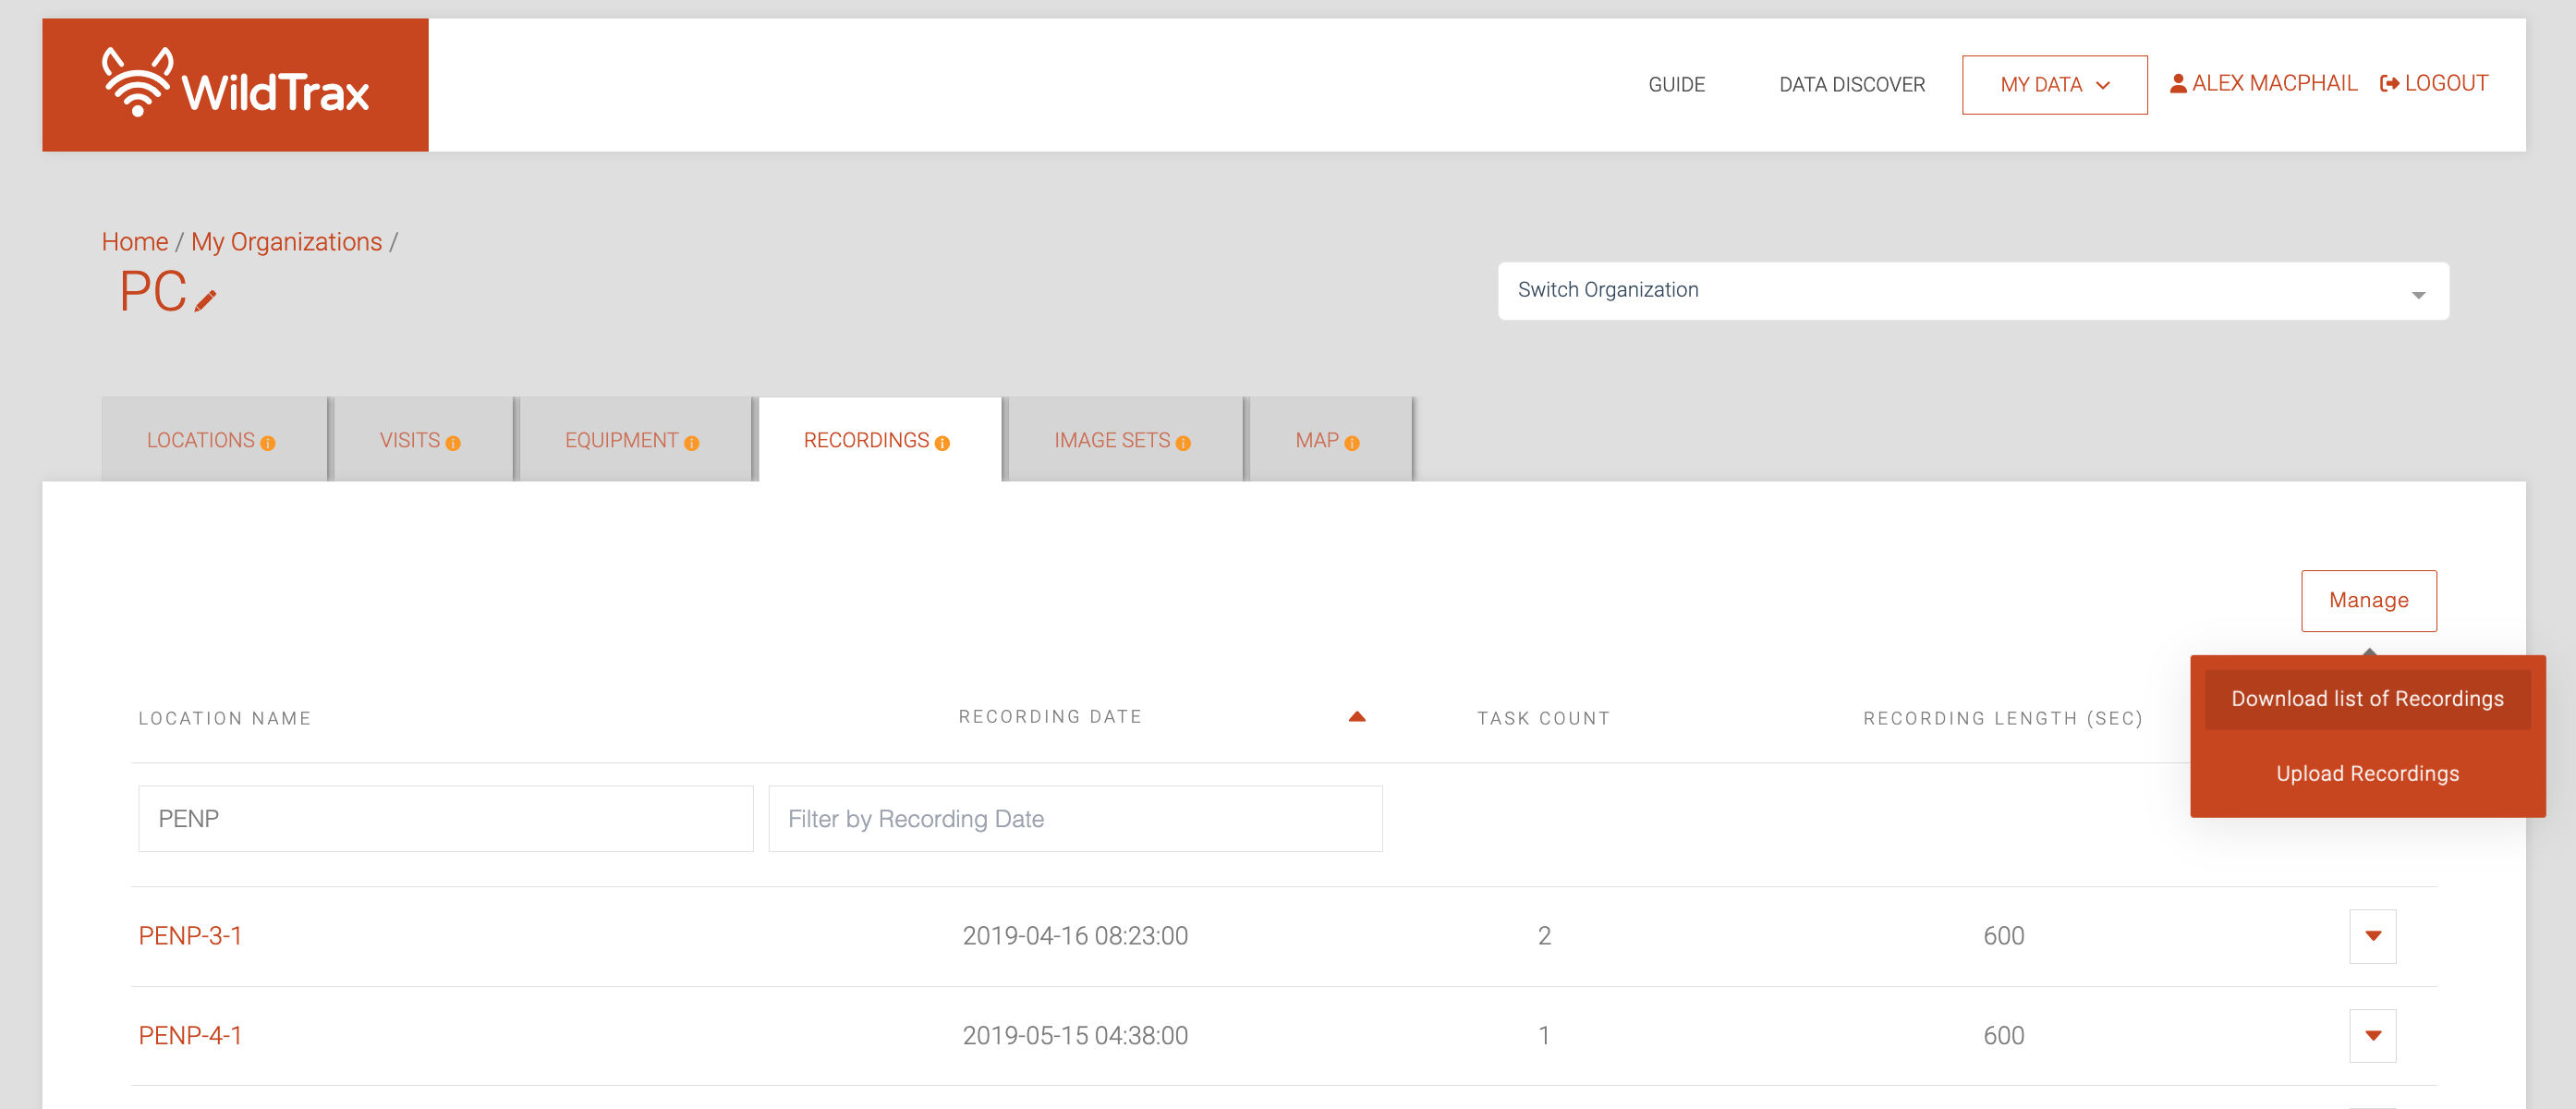
\includegraphics{download-recs.png}

}

\caption{\label{fig-download-recs}Downloading a list of recordings from
WildTrax}

\end{figure}

\hypertarget{tbl-loc-summary}{}
\begin{table}

\caption{\label{tbl-loc-summary}Locations surveyed across years. Ones indicated a deployment in that
year for that location }Location summary for ARUs deployed}
\centering
\begin{tabular}[t]{l|r|l|l}
\hline
Location & 2023 & Site & Treatment\\
\hline
AC-C2 & 1 & Alder Creek & Control\\
\hline
AC-T1 & 1 & Alder Creek & Prescribed Burn\\
\hline
AC-T2 & 1 & Alder Creek & Prescribed Burn\\
\hline
JR-C1 & 1 & Jarvis River & Control\\
\hline
JR-C2 & 1 & Jarvis River & Control\\
\hline
JR-T1 & 1 & Jarvis River & Prescribed Burn\\
\hline
JR-T2 & 1 & Jarvis River & Prescribed Burn\\
\hline
JR-T3 & 1 & Jarvis River & Prescribed Burn\\
\hline
\end{tabular}
\end{table}

\begin{figure}

\sidecaption{\label{fig-locs}ARU monitoring locations surveyed each year
as part of the songbird monitoring program.}

{\centering 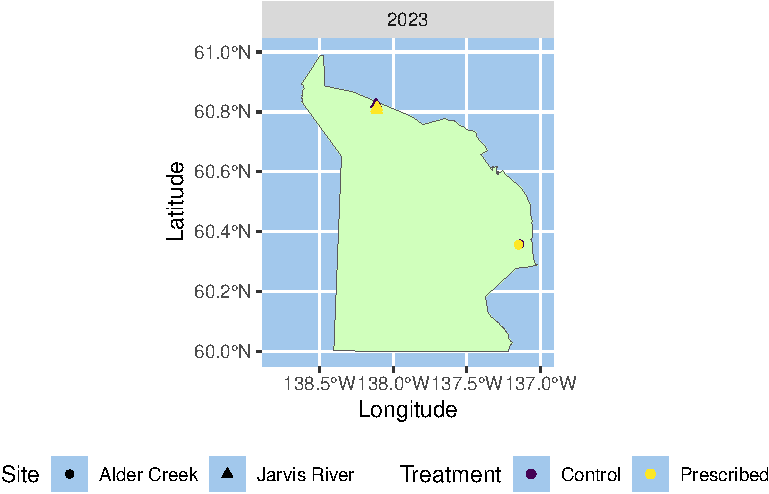
\includegraphics{knpr-pam_files/figure-pdf/fig-locs-1.pdf}

}

\end{figure}

\begin{figure}

\sidecaption{\label{fig-recs-collect}Ridgeplot of recordings collected
for each location over each survey year}

{\centering 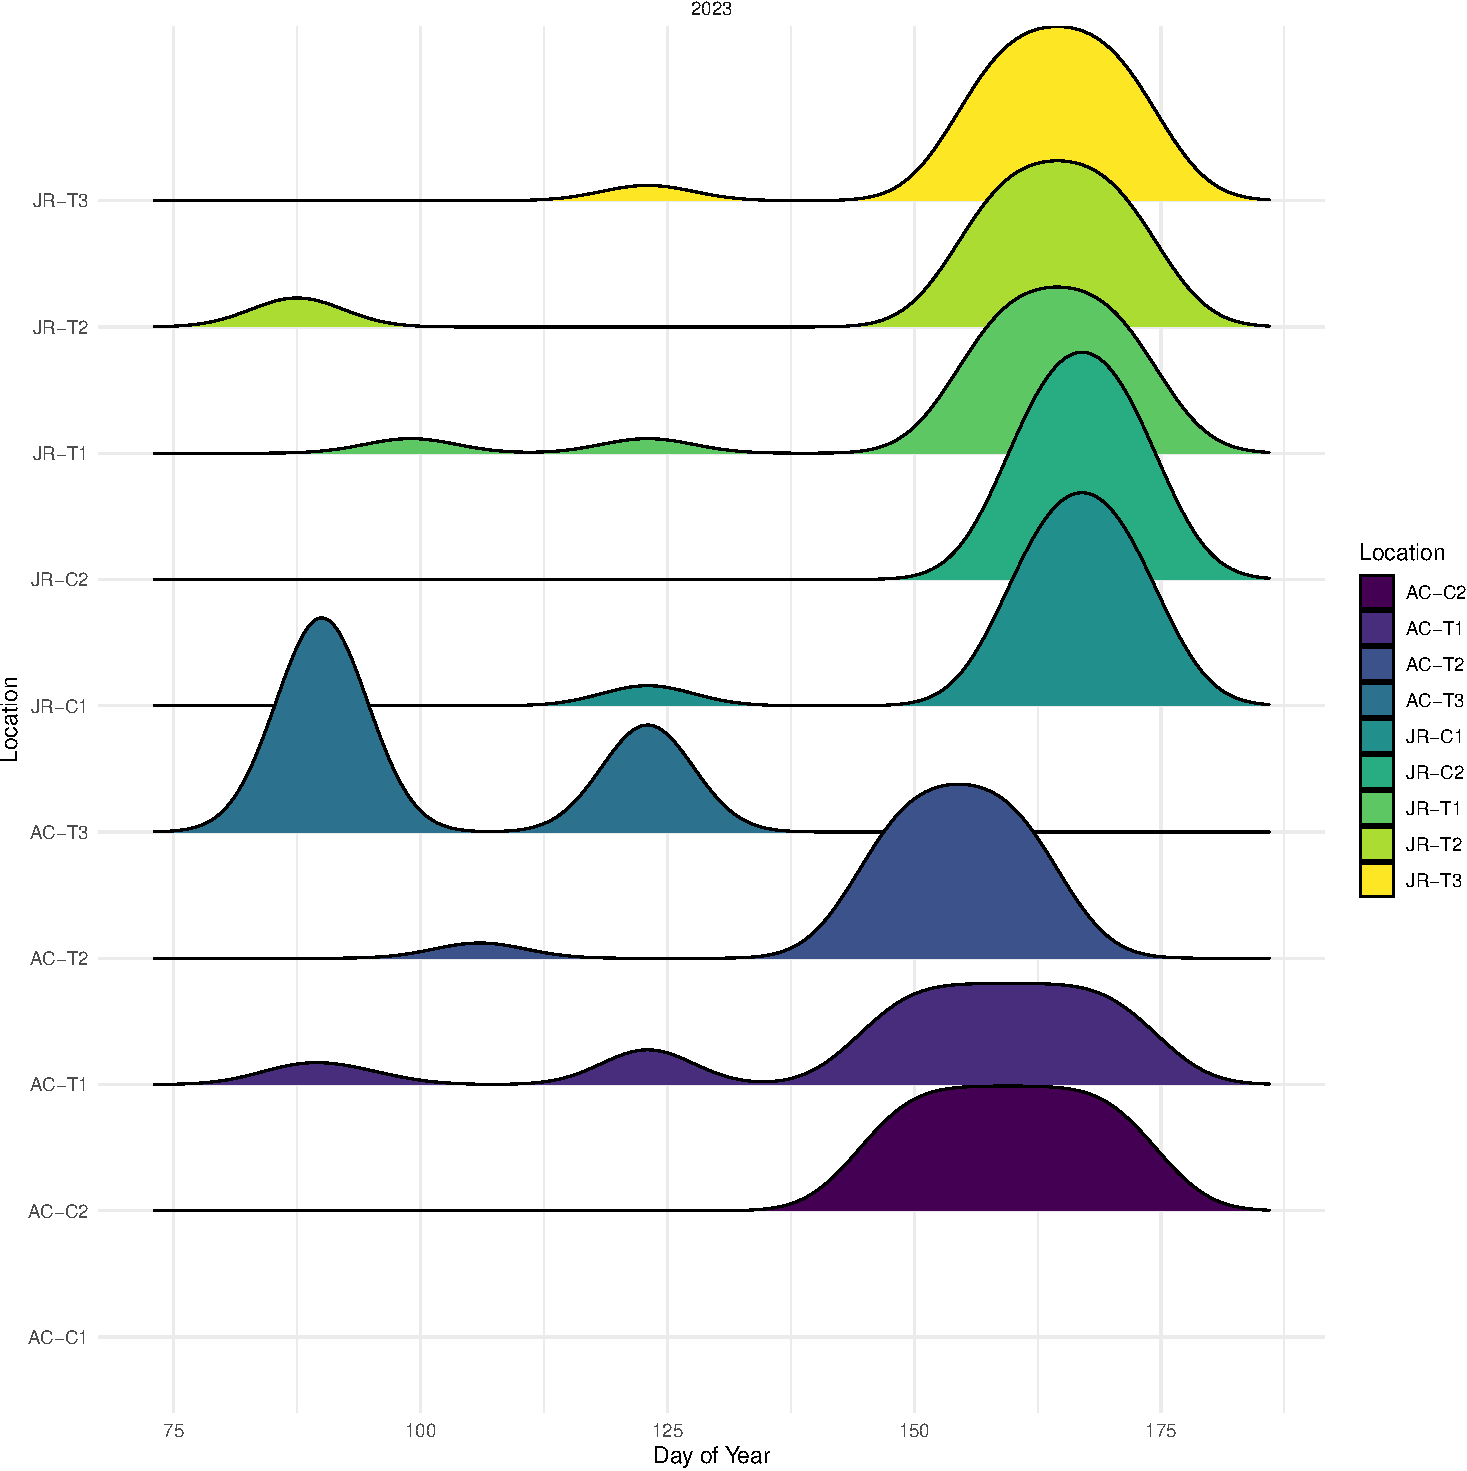
\includegraphics{knpr-pam_files/figure-pdf/fig-recs-collect-1.pdf}

}

\end{figure}

\hypertarget{community-data-processing}{%
\subsection{Community data processing}\label{community-data-processing}}

The principal goal for data processing was to describe the acoustic
community of species heard at locations while choosing a large enough
subset of recordings for analyses. To ensure balanced replication, for
each location surveyed, four randomly selected recordings were processed
for 3-minutes during the morning hours of 5:00 AM - 7:59 AM ideally on
four separate dates (see Table~\ref{tbl-loc-repl}). Four recordings will
ensure that we have the minimum number of samples for a simple occupancy
analysis (Darryl I. MacKenzie et al.
(2002)\marginpar{\begin{footnotesize}\leavevmode\vadjust pre{\protect\hypertarget{ref-mackenzie2002estimating}{}}%
MacKenzie, Darryl I, James D Nichols, Gideon B Lachman, Sam Droege, J
Andrew Royle, and Catherine A Langtimm. 2002. {``Estimating Site
Occupancy Rates When Detection Probabilities Are Less Than One.''}
\emph{Ecology} 83 (8): 2248--55.\vspace{2mm}\par\end{footnotesize}}
and Darryl I. MacKenzie et al.
(2003)\marginpar{\begin{footnotesize}\leavevmode\vadjust pre{\protect\hypertarget{ref-imperfect-occu}{}}%
MacKenzie, Darryl I., James D. Nichols, James E. Hines, Melinda G.
Knutson, and Alan B. Franklin. 2003. {``ESTIMATING SITE OCCUPANCY,
COLONIZATION, AND LOCAL EXTINCTION WHEN a SPECIES IS DETECTED
IMPERFECTLY.''} \emph{Ecology} 84 (8): 2200--2207.
https://doi.org/\url{https://doi.org/10.1890/02-3090}.\vspace{2mm}\par\end{footnotesize}}).
Tags are made using count-removal (see Farnsworth et al.
(2002)\marginpar{\begin{footnotesize}\leavevmode\vadjust pre{\protect\hypertarget{ref-farnsworth2002removal}{}}%
Farnsworth, George L, Kenneth H Pollock, James D Nichols, Theodore R
Simons, James E Hines, and John R Sauer. 2002. {``A Removal Model for
Estimating Detection Probabilities from Point-Count Surveys.''}
\emph{The Auk} 119 (2): 414--25.\vspace{2mm}\par\end{footnotesize}},
Sólymos et al.
(2018)\marginpar{\begin{footnotesize}\leavevmode\vadjust pre{\protect\hypertarget{ref-time-removal}{}}%
Sólymos, Péter, Steven M. Matsuoka, Steven G. Cumming, Diana Stralberg,
Patricia Fontaine, Fiona K. A. Schmiegelow, Samantha J. Song, and Erin
M. Bayne. 2018. {``{Evaluating time-removal models for estimating
availability of boreal birds during point count surveys: Sample size
requirements and model complexity}.''} \emph{The Condor} 120 (4):
765--86. \url{https://doi.org/10.1650/CONDOR-18-32.1}.\vspace{2mm}\par\end{footnotesize}})
where tags are only made at the time of first detection of each
individual heard on the recordings. In case a species was overly
abundant a TMTT (`too many to tag') flag was used (see
Table~\ref{tbl-tmtt}). 4\% of the total tags were TMTT but were
subsequently converted to numeric using
\texttt{wildRtrax::wt\_replace\_tmtt}. We also verified that all tags
that were created were checked by a second observer (n = 98.64\%) to
ensure accuracy of detections (see Table~\ref{tbl-verified}). Amphibian
abundance was estimated at the time of first detection using the
\href{https://www.usgs.gov/centers/eesc/science/north-american-amphibian-monitoring-program}{North
American Amphibian Monitoring Program} with abundance of species being
estimated on the scale of ``calling intensity index'' (CI) of 1 - 3.
Vocalizing mammals such as Red Squirrel, were also noted on the
recordings. After the data are processed in WildTrax, the
\href{https://abbiodiversity.github.io/wildRtrax/}{wildRtrax} package is
use to download the data into a standard format prepared for analysis.
The \texttt{wt\_download\_report} function downloads the data directly
to a R framework for easy manipulation (see
\href{https://abbiodiversity.github.io/wildRtrax/articles/apis.html}{wildRtrax
APIs}).

\hypertarget{tbl-verified}{}
\begin{table}
\caption{\label{tbl-verified}Proportion of tags verified }\tabularnewline

\centering
\begin{tabular}{l|r|r}
\hline
Tag is verified & Count & Proportion\\
\hline
 & 2 & 1.36\\
\hline
t & 145 & 98.64\\
\hline
\end{tabular}
\end{table}

\hypertarget{tbl-tmtt}{}
\begin{table}
\caption{\label{tbl-tmtt}TMTT tags }\tabularnewline

\centering
\begin{tabular}{l|l|l|l}
\hline
location & recording\_date\_time & species\_code & individual\_count\\
\hline
AC-C2 & 2023-06-06 06:30:00 & WWCR & TMTT\\
\hline
AC-T1 & 2023-06-21 07:30:00 & WWCR & TMTT\\
\hline
AC-T2 & 2023-05-27 07:30:00 & WWCR & TMTT\\
\hline
AC-T2 & 2023-06-01 05:30:00 & WWCR & TMTT\\
\hline
JR-T1 & 2023-06-21 06:30:00 & WWCR & TMTT\\
\hline
JR-T3 & 2023-06-06 07:30:00 & WWCR & TMTT\\
\hline
\end{tabular}
\end{table}

\hypertarget{tbl-loc-repl}{}
\begin{table}
\caption{\label{tbl-loc-repl}Example of tasks and unit replication for listening at PENP-4-1 }\tabularnewline

\centering
\begin{tabular}{l|r|l|l|r}
\hline
location & year & task\_duration & typ & n\\
\hline
AC-C2 & 2023 & 300s & Dawn & 4\\
\hline
AC-T1 & 2023 & 300s & Dawn & 4\\
\hline
AC-T2 & 2023 & 300s & Dawn & 4\\
\hline
JR-C1 & 2023 & 300s & Dawn & 4\\
\hline
JR-C2 & 2023 & 300s & Dawn & 4\\
\hline
JR-T1 & 2023 & 300s & Dawn & 4\\
\hline
JR-T2 & 2023 & 300s & Dawn & 4\\
\hline
JR-T3 & 2023 & 300s & Dawn & 4\\
\hline
\end{tabular}
\end{table}

\begin{center}\rule{0.5\linewidth}{0.5pt}\end{center}

\hypertarget{results}{%
\section{Results}\label{results}}

Three locations (\texttt{AC-C1}, \texttt{AC-T3}, \texttt{JR-BAT}) failed
and did not complete their intended recording schedule.

A total of 16 species were found. Figure~\ref{fig-spp-rich-locs}
describes the relationship of species richness across each location and
survey year with Figure~\ref{fig-spp-rich-annual} showing the
relationship between species richness and survey effort.

\begin{figure}

\sidecaption{\label{fig-spp-rich-locs}Species richness at forest
monitoring locations across years}

{\centering 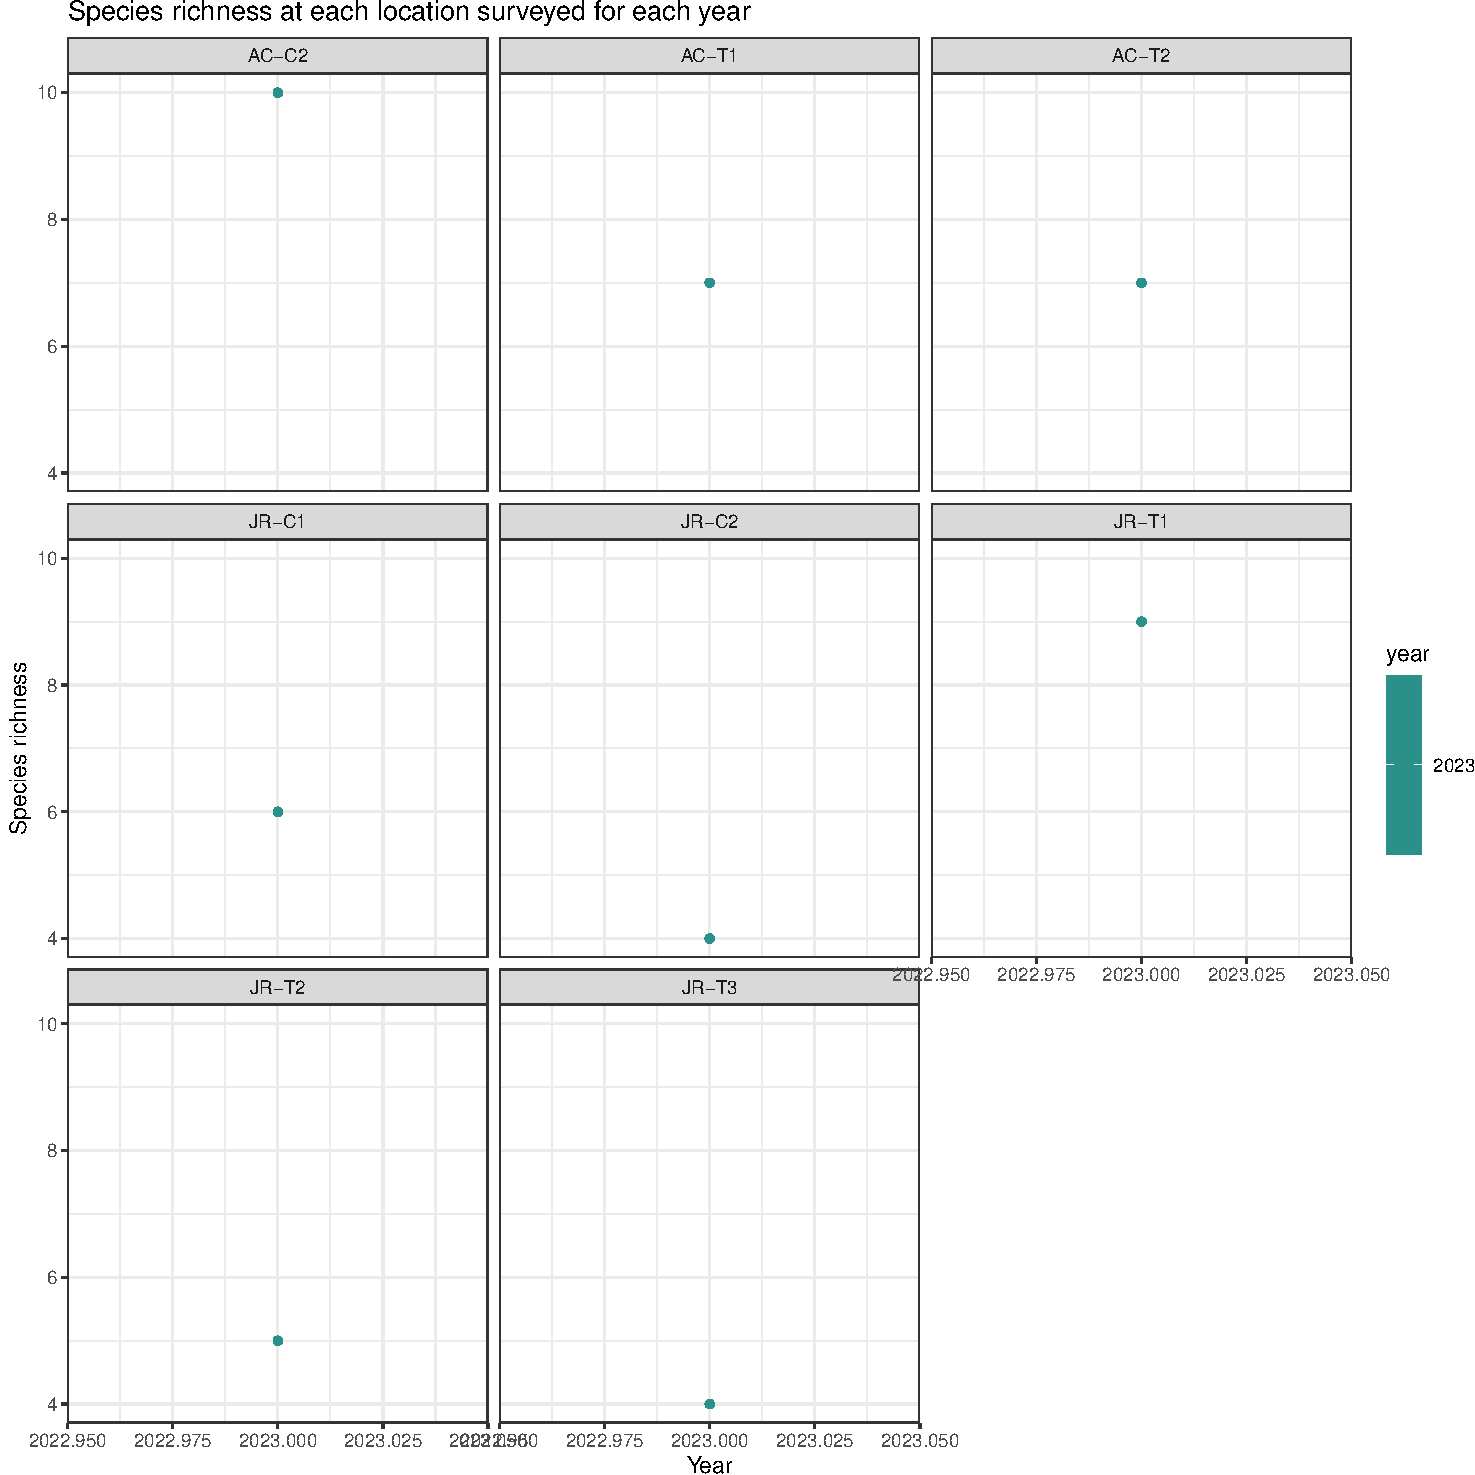
\includegraphics{knpr-pam_files/figure-pdf/fig-spp-rich-locs-1.pdf}

}

\end{figure}

\begin{figure}

\sidecaption{\label{fig-spp-rich-annual}Species richness at forest
monitoring locations across years considering sampling effort}

{\centering 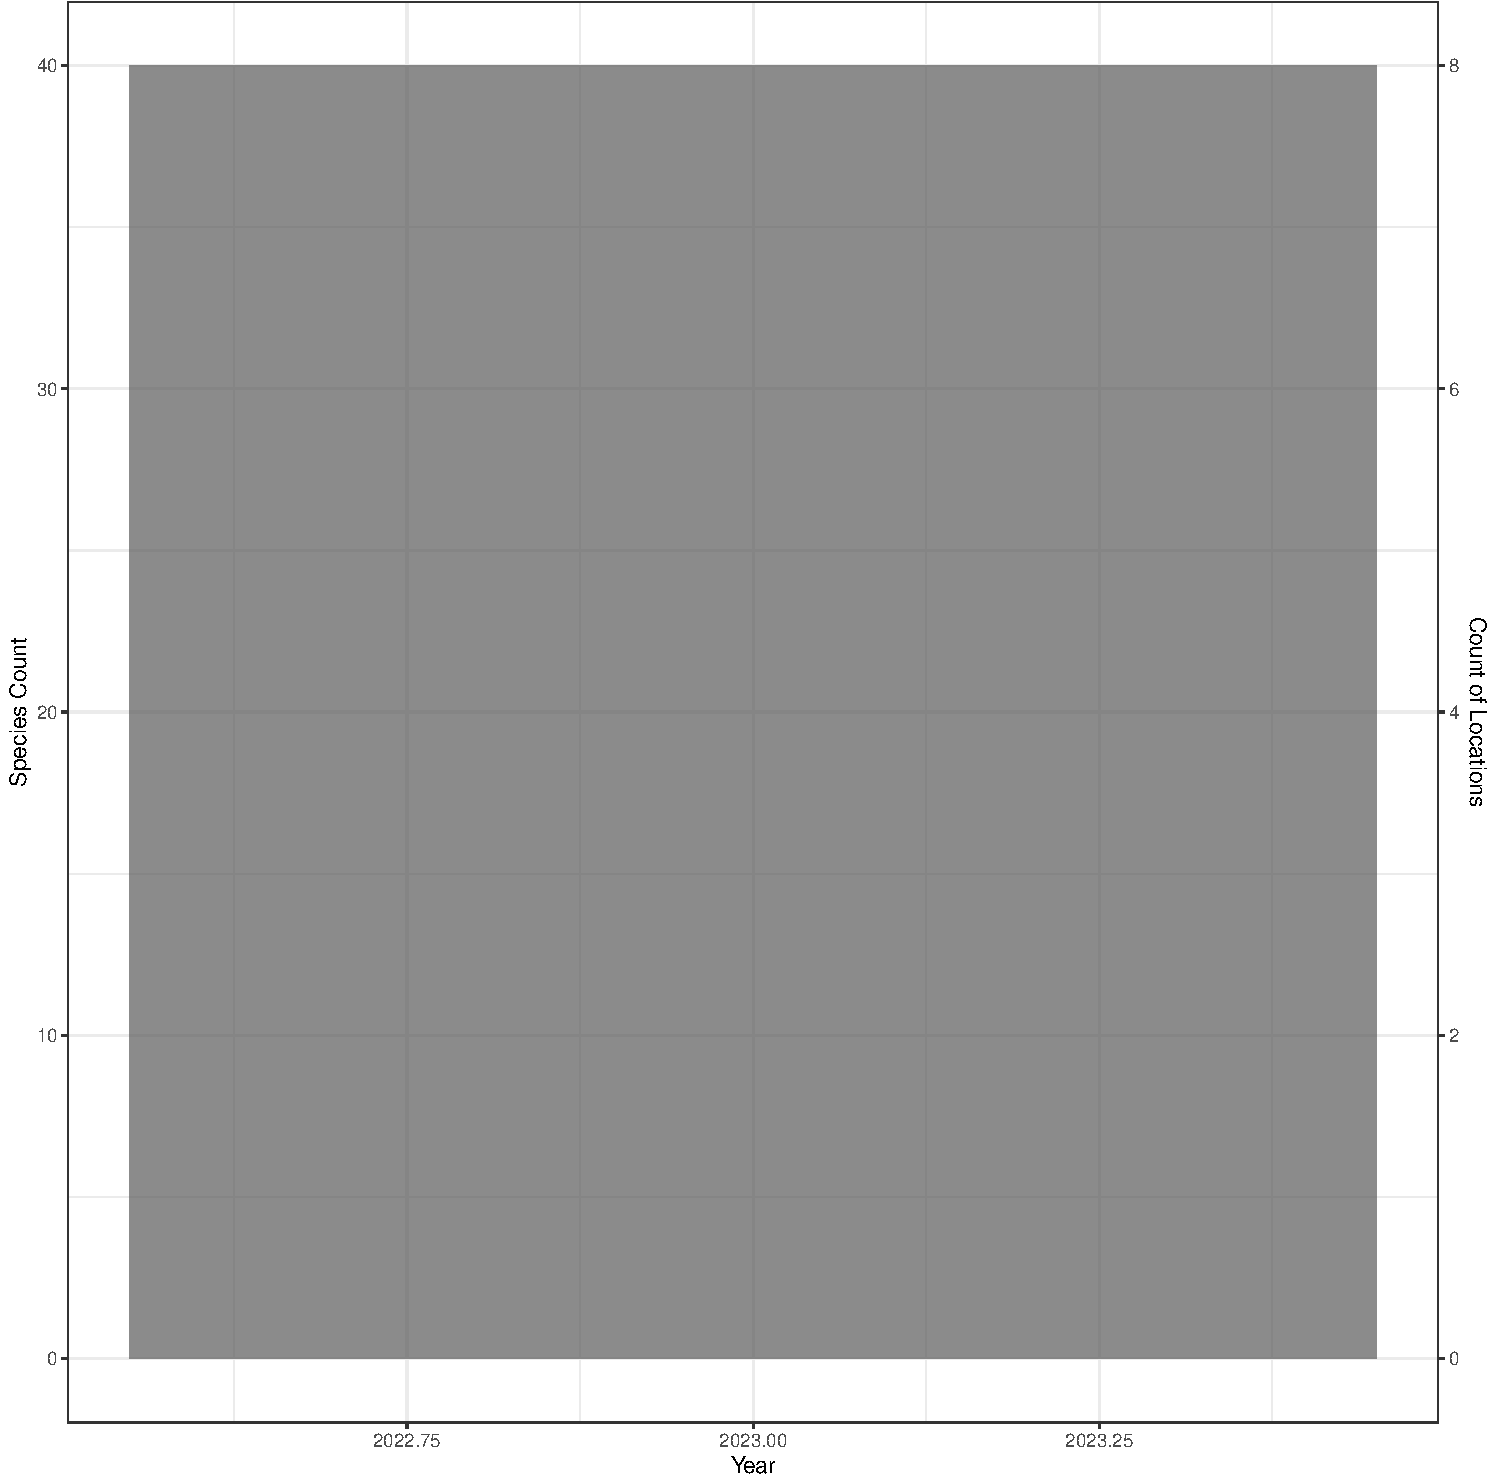
\includegraphics{knpr-pam_files/figure-pdf/fig-spp-rich-annual-1.pdf}

}

\end{figure}

\hypertarget{tbl-bird-guilds}{}
\begin{table}
\caption{\label{tbl-bird-guilds}Common bird forest species guilds. For nesting habitat; Ag =
Agricultural, Be = Beach, Bo = Bog, CW = Coniferous Woodlands, ES =
Early Successional, MW = Mixed Woodlands, OW = Open Woodlands, TSS =
Treed/Shrubby Swamp, Ur = Urban. Species from CW, MW, OW, TSS were used
for analysis. }\tabularnewline

\centering
\begin{tabular}{l|l}
\hline
species\_code & species\_common\_name\\
\hline
BOCH & Boreal Chickadee\\
\hline
CAJA & Canada Jay\\
\hline
CHSP & Chipping Sparrow\\
\hline
CORE & Common Redpoll\\
\hline
DEJU & Dark-eyed Junco\\
\hline
GCKI & Golden-crowned Kinglet\\
\hline
HETH & Hermit Thrush\\
\hline
LEYE & Lesser Yellowlegs\\
\hline
NONE & NONE\\
\hline
PIGR & Pine Grosbeak\\
\hline
PISI & Pine Siskin\\
\hline
RESQ & Red Squirrel\\
\hline
SWTH & Swainson's Thrush\\
\hline
UNPA & Unidentified Passerine\\
\hline
UNTH & Unidentified Thrush\\
\hline
VATH & Varied Thrush\\
\hline
WIWA & Wilson's Warbler\\
\hline
WWCR & White-winged Crossbill\\
\hline
YRWA & Yellow-rumped Warbler\\
\hline
\end{tabular}
\end{table}

\begin{figure}

\sidecaption{\label{fig-spp-activity}Seasonal detection activity of most
commonly detected forest species}

{\centering 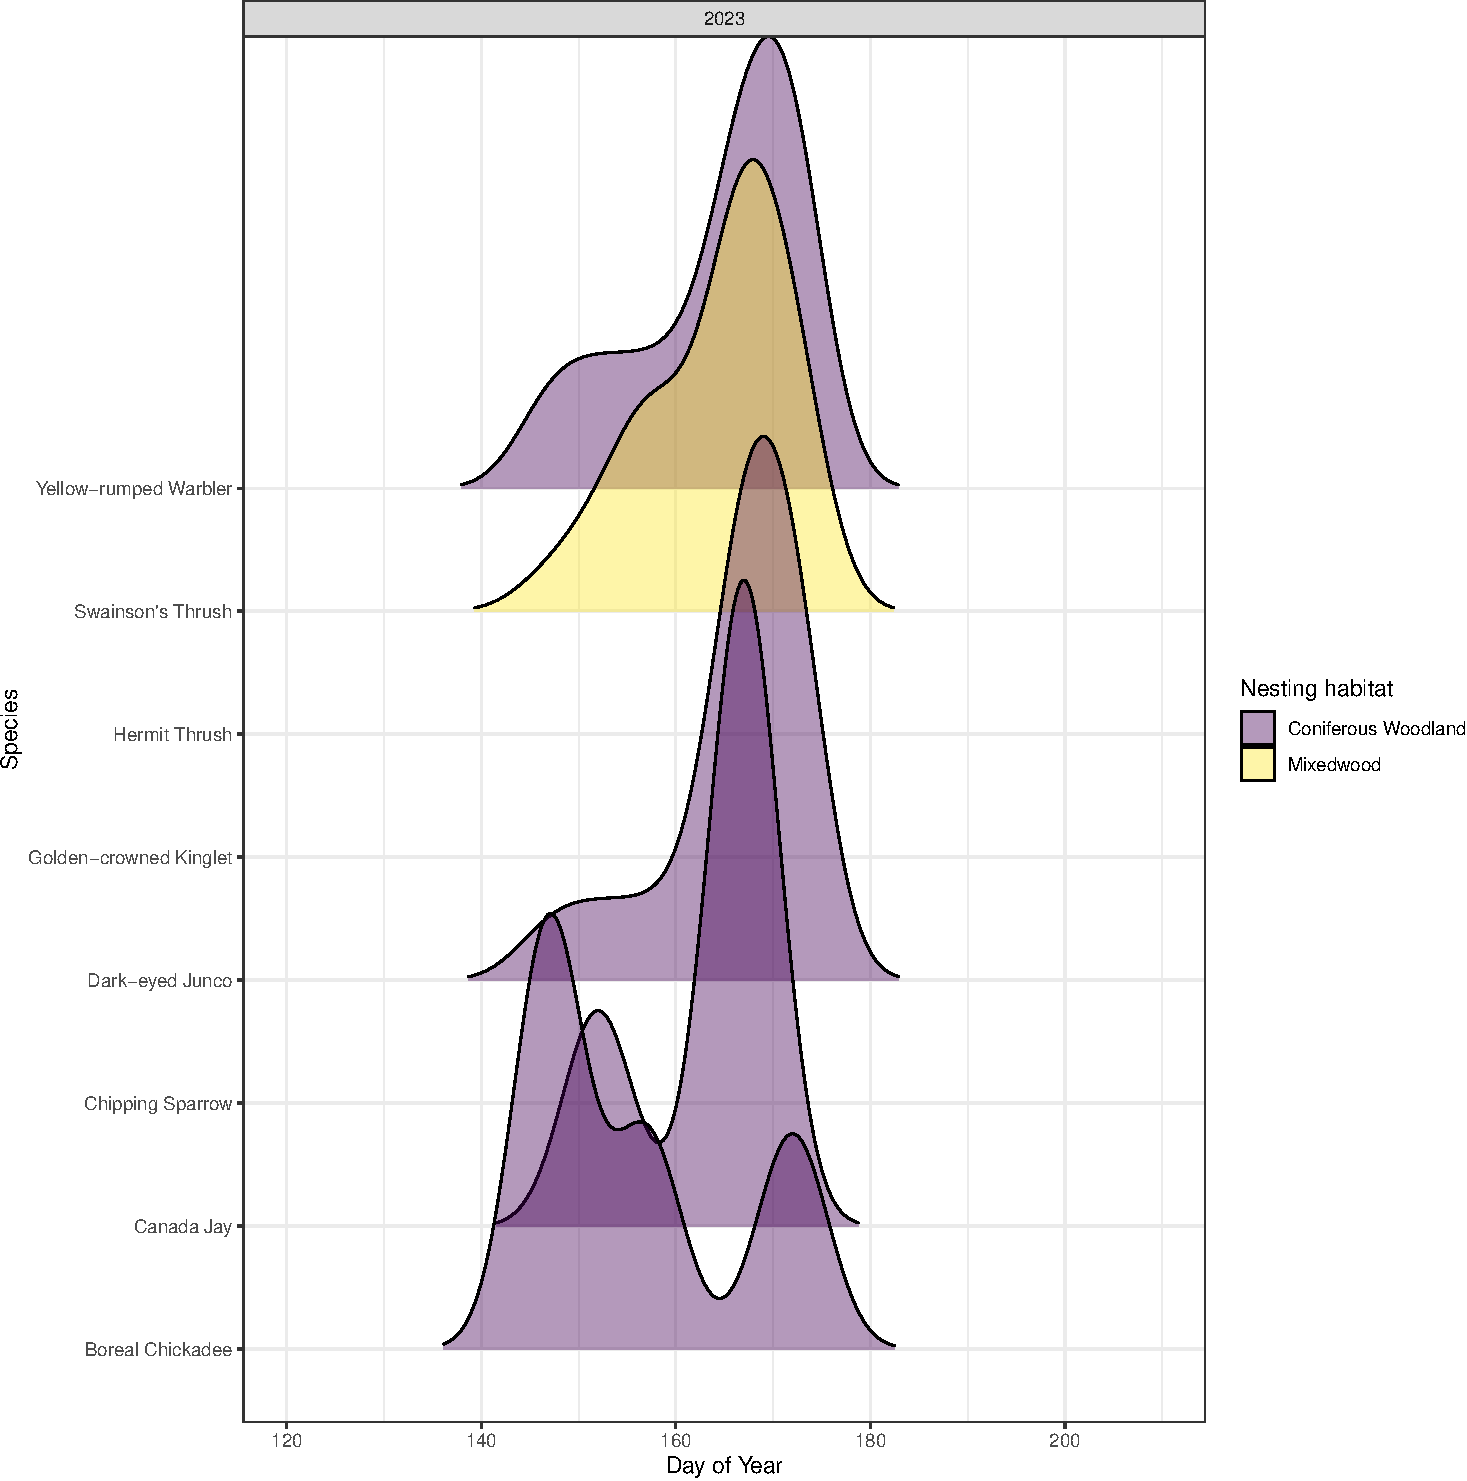
\includegraphics{knpr-pam_files/figure-pdf/fig-spp-activity-1.pdf}

}

\end{figure}

\hypertarget{discussion}{%
\section{Discussion}\label{discussion}}

While this project has yielded promising results, there are several
operational improvements necessary to fully realize its potential moving
into next season. Some key recommendations include:

\begin{itemize}
\item
  \textbf{Extending survey window and recording schedule}: Initiating
  the survey window to encompass resident and early-migrant species
  (early May) and extending it into the post-breeding season (mid-July)
  will capture a comprehensive range of species. Given the diverse
  migration timing and breeding patterns among species, extending the
  window will help enrich the data set and may provide a Recording bird
  vocalizations throughout the deployment period at various times of the
  day--pre-dawn, dawn, post-dawn, pre-dusk, dusk, post-dusk, and
  night--enables a comprehensive assessment of bird diversity and
  activity patterns. Birds exhibit diverse diurnal and nocturnal
  behaviors, with some species being more vocal during specific times of
  the day or night. Continuous recording across different times allows
  ARUs to capture a broad spectrum of species, including those that are
  crepuscular or nocturnal, providing valuable insights into their
  behaviors and habitat preferences. This approach enhances the accuracy
  and completeness of bird surveys, offering valuable data for planning
  and management efforts.
\item
  \textbf{Equipment maintenance and management}: Given that 3 locations
  failed during their deployment, ensuring that equipment is properly
  functioning, tested and maintained prior to deployment is crucial for
  ensuring the success of a long-term monitoring program. The ABMI
  provides
  \href{https://ftp-public.abmi.ca/home/publications/documents/599_ABMI_2021_TerrestrialARUandRemoteCameraTrapProtocols_ABMI.pdf}{Equipment
  Protocols} to help assist in the maintenance and deployment of most
  \href{https://www.wildlifeacoustics.com/}{Wildlife Acoustics} makes
  and models. Most importantly, ensure the units are cleaned and
  inspected for physical or mechanical damage, update the firmware and
  conduct tests to ensure functionality in a controlled environment.
\item
  \textbf{Localized Monitoring}: Consistently deploying ARUs in the same
  locations on the landscape year after year will help to establish
  robust monitoring sites. By continuously surveying specific areas,
  changes in bird distribution and abundance can be monitored. This
  approach facilitates the identification of long-term trends and
  enables the understanding of changes in bird populations and guilds
  over time, especially with planned changes with the prescribed burns.
\item
  \textbf{ARU deployment in prescribed burns}: Deploying at least one
  ARU per 0.5 hectares burned ensures thorough monitoring of post-burn
  effects on bird populations. This density of ARU deployment generates
  detailed data on how bird populations respond to habitat changes
  following prescribed burns, facilitating the understanding of
  ecosystem resilience and recovery processes. By monitoring post-burn
  effects on bird populations, researchers can inform conservation
  strategies aimed at mitigating the impact of habitat disturbance.
\item
  \textbf{Bat monitoring enhancements}: Continuing to use a sample rate
  to 256 kHz is advisable, given that bat species in western Canada
  typically do not vocalize beyond this frequency range. The sampling
  rate will optimize the total amount of data volume collected.
  Programming the Max Time Between Calls (TBC) by adjusting the trigger
  window from 3 to 2 seconds. The
  \href{https://www.nabatmonitoring.org/}{North American Bat Monitoring
  Program} offers many additional recommendations for deployment,
  processing and interpretation of ultrasonic data.
\end{itemize}




\end{document}
